\documentclass[12pt,a4paper]{article}
  \usepackage[latin1]{inputenc}
  \usepackage[T1]{fontenc} 
  \usepackage[francais, english]{babel} 
  \usepackage{amsmath, amsthm}
\newtheorem{proposition}{Proposition}
\newtheorem{lemma}{Lemma}
\newtheorem*{proof*}{Proof}

\newtheorem{remark}{Remark}

\usepackage[a4paper,left=2cm, right=2cm,top=3cm,bottom=3cm]{geometry}

  \usepackage{amssymb,amsfonts}
  \usepackage{mathrsfs}
  \usepackage{color}
  %\usepackage{hyperref}
	\usepackage{dsfont}
	\usepackage{graphicx}
	\usepackage{algorithmicx}
    \usepackage[ruled]{algorithm}
    \usepackage{algpseudocode}
     \usepackage{marginnote}
\newcommand{\Ptr}{\mathcal P^{\rm tr}}
\newcommand{\tr}{{\rm tr}}
\newcommand{\N}{\mathbb N}
\newcommand{\calK}{\mathcal K}
\newcommand{\calH}{\mathcal H}
\newcommand{\calP}{\mathcal P}
\newcommand{\R}{\mathbb R}
\newcommand{\Ktr}{\calK^{\rm tr}}
  \title{ \bfseries \Huge {Optimal greedy parameter selection in the reduced basis context}} 
  \author{  \scshape  Amina Benaceur }
 \date{\today}       
  \sloppy         
  \newcommand\red[1]{\textcolor{red} {#1} }
  \begin{document}
  \maketitle
  \section{Basic notation}
  Let us also introduce a continuous linear form $ f: X\rightarrow \mathbb{R}$ and a family of symmetric continuous bilinear forms  
  $ a: X\times X \times \mathcal P  \rightarrow \mathbb{R}$. We assume that $a$ is symmetric, i.e.
$a(v,w;\mu)=a(w,v;\mu)$, $\forall w,v \in X,\ \forall \mu \in D$; and coercive:
$\exists \alpha_{0}>0, \forall \mu \in D, \alpha_{0} \leq \alpha(\mu) = \inf_{w \in X}
\frac{a(w,w;\mu)}{\|w\|^{2}_{X}}$.
  In all that follows, $<\cdot,\cdot>$ denotes a suitable inner product, for instance that of $ L^2(\Omega)$
  and $\|\cdot\|_X$ is the corresponding norm. 
  Consider the elliptic parameter-dependent problem: find $u(\mu) \in X$ s.t.
  \begin{equation}\label{pde}
   a(u(\mu),w;\mu) = f(w),\ \ \ \forall w \in X.
  \end{equation}
The reduced basis method has been introduced for the sake of addressing such parameter-dependent problems.

A key purpose is to select the best parameters that would lead 
to an optimal reduced order model.

\section{The strong greedy algorithm}
Let $\calH$ be a Hilbert space of real-valued functions defined on a spatial domain $\Omega \subset \R^d$, where $d\in \N^*$, and let $\calK\subset\calH$ be a compact set. The Hilbert space $\calH$ is endowed with an inner product $(\cdot,\cdot)$ and a norm $\|\cdot\|$. For a subspace $X\subset\calH$, we introduce the projector $\Pi_X$ onto $X$.
Finally, we consider a discrete training parameter set $\Ptr\subset\calP$. Greedy algorithms have been widely investigated in the literature to select parameter values.
Their main purpose is seeking a collection of functions $\{u(\mu_1),\ldots,u(\mu_n)\}$ that produces accurate approximations of all functions $f\in\calP$. The key idea of the greedy algorithm is to create a set of hierarchical spaces
$X_1\subset X_2\subset\cdots\subset X_n\subset\cdots\subset \calK$, with $\mathrm{dim}(X_n) = n$, that are progressively enriched by a function $h\in\Ktr$ that maximizes a given error.

To start with, we select a function 
\begin{equation}
h_1 = \underset{h\in\Ktr}{\rm max}\|h\|,
\end{equation}
and we define the first approximation space
\begin{equation}
 X_1 = {\rm span}\{h_1\}.
\end{equation}
The following approximation spaces are defined by induction. 
At each new iteration $n>1$, we select the worst approximated function in $X_{n-1}$, i.e.
\begin{equation}
h_n = \underset{h\in\Ktr}{\rm max}\|h-\Pi_{X_{n-1}}h\|,
\end{equation}
and we define the new approximation space
\begin{equation}
 X_n = X_{n-1} + {\rm span}\{h_n\}.
\end{equation}
The greedy algorithm is summarized in Algorithm~\ref{alg:strong}.

 \begin{algorithm}[H]
\caption{Greedy algorithm}\label{alg:strong}
\begin{algorithmic}[1]
\Statex \textbf{\underline{Input :}}
\ $\Ptr$ : training set
\Statex\qquad\qquad $\epsilon$ : threshold
\State Search $\mu_1 = \underset{\mu\in\Ptr}{\rm max}\|u(\mu)\|$
\State Set $X_1 = {\rm span}\{u(\mu_1)\}$
\While{ $>\epsilon$}
\State Search $\mu_{n+1} = \underset{h\in\Ptr}{\rm max}\|u(\mu)-\Pi_{X_{n-1}}u(\mu)\|$
\State Set $X_{n+1} = X_n+ {\rm span}\{u(\mu_{n+1})\}$
\EndWhile
\Statex \textbf{\underline {Output :}}
$ X_N$ : reduced space
\Statex \qquad\qquad\ \ ${N}$ : dimension of the final space
\vspace{0.2cm}
\end{algorithmic}
\end{algorithm}
We emphasize that the sequence of selected functions $(h_1,\ldots,h_N)$ is not unique thereby implying the non-uniqueness of the error sequence $(e_1,\ldots,e_N)$, where $e_n = \underset{h\in\Ktr}{\rm max}\|h-\Pi_{X_{n-1}}h\|$, for $n\in\{1,\ldots,N\}$.

\section{Towards selection uniqueness}
The goal of this section is to ensure the uniqueness of the selection resulting from the greedy algorithm. 
Given a reduced subspace $X_{n-1}$, assume that
\begin{equation}
\exists\ h_n^1, \ldots, h_n^I\in\Ktr: \ 
h_n^1, \ldots, h_n^I\in \underset{h\in\Ktr}{\rm argmax}\|h-\Pi_{X_{n-1}}h\|,
\end{equation}
for an integer $I\geq 2$.
In the standard setting where the choice among $h_n^1,\ldots,h_n^I$ is made randomly, the sequence of errors $(e_1,\ldots,e_N)$ will differ accordingly. In view of a fast decay of the sequence of errors, we suggest to decide on the selection based on the following criterion
\begin{equation}
 h_n^i\in\underset{1\leq i\leq I}{\rm argmin}\ \underset{h\in\Ktr}{\rm max}\|h-\Pi_{X_{n-1}+{\rm span}\{h_n^1\}}h\|
\end{equation}


\section{Predictive greedy algorithm}
The elements that span a reduced space in the reduced basis method
 are usually selected by means of standard greedy algorithms~\cite{pate,haasdonk13}.
The selection strategy that is commonly proposed in the literature is that of enriching the current space with the vector corresponding to the worst approximated parameter, i.e.
 \begin{equation}\label{std_greedy}
  \mu_{n+1} = \underset{\mu \in \mathcal P}{\mathrm{argmax}}\ \|u(\mu)-P_N u(\mu)\|_X
 \end{equation}
where $P_N$ is the orthogonal projection onto the current reduced subspace $X_{N}\subset X$.
 Nevertheless, were we to seek an optimal selection among the available vectors, the criterion would be different.
 Given a parameter value $\mu\in\calP$ and a linear subspace $X_N$ of dimension $N$, we introduce the linear subspace $X^\mu_{n+1}$ of dimension $n+1$ defined as follows 
\begin{align*}
X^\mu_{n+1} &= X_N + \mathrm{span}\{u(\mu)\} \\
&=X_N + \mathrm{span}\{\theta_{n+1}(\mu)\} 
\end{align*}
with
\begin{align*}
\theta_{n+1}(\mu) = \frac{1}{\| u(\mu) - P_N u(\mu) \|_X} \big( u(\mu) - P_N u(\mu) \big).
\end{align*}
Additionally, we introduce the operator $P^\mu_{n+1}$ as the orthogonal projection on the subspace $X^\mu_{n+1}$.
 
 \begin{proposition}
Given a linear subspace $X_N\subset X$, the optimal greedy parameter selection within the discrete parameter set $\calP^\tr$ at stage $n+1$ is given by
\end{proposition}
 \begin{equation}\label{mod_greedy}
  \mu_{n+1} \in \underset{\mu \in \calP^\tr}{\mathrm{argmin}} \underset{\nu \in \calP^\tr} {\mathrm{\ sup\ }}\|u(\nu)- P^\mu_{n+1} u(\nu)\|_X
 \end{equation}

\begin{proof}
By construction, it holds that 
$$
\forall \eta\in\calP^\tr, \qquad\underset{\nu \in \calP^\tr} {\mathrm{\ sup\ }}\|u(\nu)- P^{\mu_{n+1}}_{n+1} u(\nu)\|_X
\leq
\underset{\nu \in \calP^\tr} {\mathrm{\ sup\ }} \|u(\nu)- P^\eta_{n+1} u(\nu)\|_X.
$$
\end{proof}

The resulting linear subspaces $X_1,\ldots,X_N$ are optimal considering a selection that is restricted to the discrete training parameter space $\Ptr$. We emphasize that they are not optimal in the sense of the Kolmogorov $N$-width: here, optimality is defined among all the 
linear $N$-dimensional subspaces of $X$ that can be spanned by available elements of the solution manifold associated to~\eqref{pde}. 
\begin{remark}
We present a simple example illustrating the suboptimality of the standard greedy criterion~\eqref{std_greedy}.
Consider $\mathbb R^3$ endowed with its canonical scalar product and a solution manifold 
$ \mathcal M = \{e_1=(1,0,0),\ e_2 = (0,1+\epsilon,0),\ e_3 = (0,0,1-\epsilon),\
e_4 = \sqrt 2^{-1}(0,1,1)\}$ with $\epsilon \in [0, 3-2\sqrt 2[$.
Let $X_1= \mathrm{span}\{e_1\}$ be an initial reduced basis space. The strong greedy algorithm enriches $X_1$ using $e_2$ through $X_2 = X_1 + \mathrm{span}\{e_2\}$, leading to 
$\mathrm{dist}(X_2,\mathcal M) = 1-\epsilon$. Nonetheless, opting for $\tilde X_2 = X_1 + \mathrm{span}\{e_4\}$
produces a better reduced basis approximation since it yields $\mathrm{dist}(\tilde X_2,\mathcal M) = 
{\sqrt{2}}^{-1}(1+\epsilon)$.
\end{remark}

\begin{proposition}
The optimal greedy selection criterion~\eqref{mod_greedy} is equivalent to
\begin{equation}
  \mu_{n+1} \in \underset{\mu \in \calP^\tr}{\mathrm{argmin}}
  \underset{\nu \in \calP^\tr} {\mathrm{\ sup\ }}
  \bigg( \|e_N(\nu)\|_X^2 -\frac{<e_N(\nu), e_N(\mu)>^2}{\|e_N(\mu)\|_X^2} \bigg)
 \end{equation}
\end{proposition}

\begin{proof}
A direct expansion of the error norm appearing in \eqref{mod_greedy} gives
  \begin{align*}
   \|u(\nu)- P^\mu_{n+1} u(\nu)\|^2_X  =& \ \|u(\nu)-P_N u(\nu)-<u(\nu),\theta_{n+1}(\mu)>\theta_{n+1}(\mu)\|^2_X \\
 =&\ \|u(\nu)-P_N u(\nu)\|_X^2 \ + <u(\nu),\theta_{n+1}(\mu)>^2  \\
 &- 2 <u(\nu),\theta_{n+1}(\mu)><u(\nu)-P_N u(\nu),\theta_{n+1}(\mu) > 
  \end{align*}
Henceforth, we set $e_N(\nu) = u(\nu)-P_N u(\nu),$ for all $\nu \in \mathcal P$. Besides, notice that
 \begin{align}\label{ortho}
  <u(\nu),\theta_{N+1}(\mu)>\ =\ <e_n(\nu),\theta_{n+1}(\mu)>.
 \end{align}
This latter equality \eqref{ortho} implies:
 \begin{align}\label{err_est}
 \|u(\nu)- P^\mu_{N+1} u(\nu)\|_X   &= \|e_n(\nu)\|_X^2 -\frac{1}{\|e_n(\mu)\|_X^2} <e_n(\nu), e_n(\mu)>^2 
   \end{align}
 Consequently, the optimal choice of the parameter $\mu_{N+1}$ resulting from \eqref{mod_greedy} is 
\begin{equation*}
  \mu_{N+1} \in \underset{\mu \in \calP^\tr}{\mathrm{argmin}}
  \underset{\nu \in \calP^\tr} {\mathrm{\ sup\ }}
  \bigg( \|e_n(\nu)\|_X^2 -\frac{<e_n(\nu), e_n(\mu)>^2}{\|e_n(\mu)\|_X^2} \bigg)
 \end{equation*}
 \end{proof}
 
 \begin{algorithm}[H]
\caption{Predictive greedy algorithm}\label{alg:predictive}
\begin{algorithmic}[1]
\Statex \textbf{\underline{Input :}}
\ $\Ptr$ : training set
\Statex\qquad\qquad $\epsilon$ : threshold
\State Search $\mu_1 = \underset{\mu\in\Ptr}{\rm argmax}\|u(\mu)\|$
\State Set $X_1 = {\rm span}\{u(\mu_1)\}$
\While{ $>\epsilon$}
\State Search $ \mu_{N+1} \in \underset{\mu \in \calP^\tr}{\mathrm{argmin}}
  \underset{\nu \in \calP^\tr} {\mathrm{\ sup\ }}
  \bigg( \|e_n(\nu)\|_X^2 -\frac{<e_n(\nu), e_n(\mu)>^2}{\|e_n(\mu)\|_X^2} \bigg)$
\State Set $X_{n+1} = X_n + {\rm span}\{\mu_{n+1}\}$
\EndWhile
\Statex \textbf{\underline {Output :}}
$X_N$ : reduced space
\Statex \qquad\qquad\ \ ${N}$ : dimension of the final space
\vspace{0.2cm}
\end{algorithmic}
\end{algorithm}


\section{Ideas}
\red{
\begin{enumerate}
\item Prove that the criterion is decreasing.
\item Look-ahead reduced set of parameters, implying a complexity $N\times M$ instead of $N^2$.
\item Second reduction step after we've done the first step using the strong greedy algorithm. It implies a squeezing of the basis and possibly spares some vectors.
\item Implement some non-coercive cases where the impact would be even more beneficial.
\item The projection error can be replaced by the RB error $\hat u(\mu) - u(\mu).$
\item Ensure the uniqueness of the hierarchical spaces resulting from the greedy algorithm using the predictive criterion.
\item A posteriori reordering of the reduced basis
\item Next step will be to do the same for the CPG algorithm.
\end{enumerate}
}

\section{Numerical results}
This section aims at testing the performances of the predictive greedy algorithm compared to the strong greedy algorithm.
Let $\mathcal P = [0,20]$ be a parameter set and $\mathcal P^{\rm tr}=\{i|0\leq i\leq 20\}$ a chosen training set.
We consider a spatial domain $\Omega\in\mathbb R^2$,  of height $H = 2$m in $y$ and length $L=4$m in $x$.
We build our training solution manifold using the partial differential equation $0.1\mu\Delta u(\mu)+\sqrt{\mu}u(\mu) = 1$, with homogeneous Neumann boundary conditions on $y = 0$ and $x = 0$, and Dirichlet boundary conditions $u(\cdot,H) = u(L,\cdot) = 1$. We perform both the strong greedy algorithm and the predictive algorithm whose accuracy is displayed in Figure~\ref{fig:err}.
\begin{figure}
 \centering
 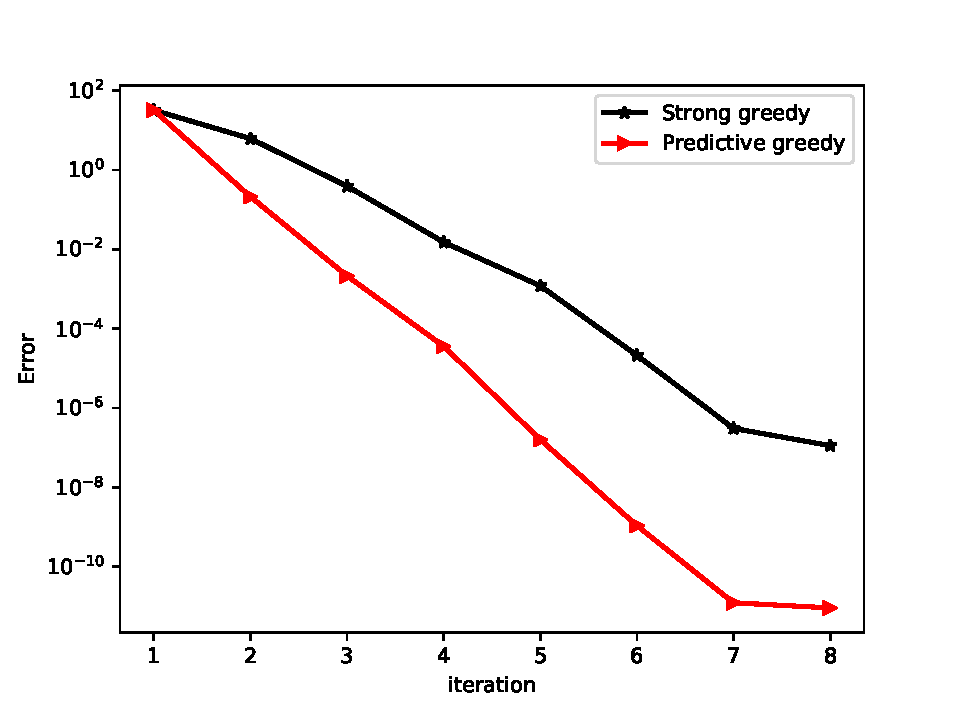
\includegraphics[width=.6\textwidth]{images/error_sg_pg.pdf}
 \caption{Evaluation of the error 
 $e_n(\mu) = {\max}_{\mu\in\mathcal P^{\rm tr}}\|u(\mu)-P_{X_n}u(\mu)\|_{\ell^\infty(\Omega^{\rm tr})}$.}
 \label{fig:err}
\end{figure}
 
   \bibliographystyle{plain}
  \bibliography{bibli}
  \end{document}
